\chapter{Giới thiệu}
\label{Chapter1}

%Tóm tắt luận văn được trình bày nhiều nhất trong 24 trang in trên hai mặt giấy, cỡ chữ Times New Roman 11 của hệ soạn thảo Winword hoặc phần mềm soạn thảo Latex đối với các chuyên ngành thuộc ngành Toán.

%Mật độ chữ bình thường, không được nén hoặc kéo dãn khoảng cách giữa các chữ.
%Chế độ dãn dòng là Exactly 17pt.
%Lề trên, lề dưới, lề trái, lề phải đều là 1.5 cm.
%Các bảng biểu trình bày theo chiều ngang khổ giấy thì đầu bảng là lề trái của trang.
%Tóm tắt luận án phải phản ảnh trung thực kết cấu, bố cục và nội dung của luận án, phải ghi đầy đủ toàn văn kết luận của luận án.
%Mẫu trình bày trang bìa của tóm tắt luận văn (phụ lục 1).

\noindent \textit{Trong chương này, đầu tiên nhóm chúng em phát biểu về bài toán đề xuất sản phẩm cũng như là ý nghĩa của nó đối với cuộc sống hiện nay. Sau đó, nhóm chúng em trình bày về vấn đề thiên lệch dữ liệu, một thách thức lớn của bài toán đề xuất sản phẩm. Từ đó dẫn đến phương pháp nhóm chúng em tìm hiểu ``Inverse Propensity Scoring'' (IPS) để khắc phục vấn đề thiên lệch dữ liệu này. Ngoài ra, ở cuối chương nhóm chúng em sẽ trình bày về cách tổ chức của khóa luận.}

\section{Phát biểu bài toán}
Ngày nay, các loại sản phẩm phục vụ cho đời sống con người được sinh ra ngày một nhiều. Điều này tạo nên thách thức cho người dùng là làm thế nào để có thể tìm thấy được các sản phẩm phù hợp với bản phân giữa một lượng sản phẩm khổng lồ như vậy. Do đó hệ thống đề xuất sản phẩm đã ra đời nhằm mục đích hỗ trợ cho người dùng trong quá trình tìm kiếm sản phẩm phù hợp cho bản thân.

Các hệ thống đề xuất sản phẩm giúp cho trải nghiệm của người dùng được cá nhân hóa, giúp tiết kiệm thời gian cho người dùng trong việc lựa chọn sản phẩm. Mặt khác, đối với các công ty nó còn tăng cao lợi thế cạnh tranh, kích thích nhu cầu mua sắm của người dùng bằng các gợi ý sản phẩm. Có thể kể đến các hệ thống đề xuất sản phẩm nổi tiếng như: hệ thống đề xuất phim của Netflix, hay hệ thống đề xuất video của Youtube, hệ thống đề xuất nhạc của Spotify và nhiều loại hệ thống đề xuất khác nữa.

Bài toán hệ thống đề xuất sản phẩm sẽ được phát biểu như sau (hình \ref{fig:chap1_rs} minh hoạ về cách thức hoạt động của hệ thống đề xuất phim):
\begin{itemize}
    \item Đầu vào là dữ liệu về điểm đánh giá của các người dùng đối với các sản phẩm trong hệ thống; dữ liệu này sẽ được đưa vào mô hình dưới dạng một ma trận tương tác thưa với mỗi dòng là các đánh giá của người dùng cho các sản phẩm. Ngoài ra, còn có thể có thêm dữ liệu về thông tin của mỗi người dùng và mỗi sản phẩm; dữ liệu này được đưa vào mô hình dưới dạng ma trận thuộc tính của người dùng và ma trận thuộc tính của sản phẩm, các điểm dữ liệu trong ma trận thuộc tính sẽ được tiền xử lý thành dạng số.

    \item Yêu cầu: đề xuất các sản phẩm trong hệ thống mà phù hợp với sở thích của mỗi người dùng (để có thể đề xuất thì một cách làm phổ biến là dự đoán điểm đánh giá của người dùng đối với các sản phẩm mà người dùng chưa đánh giá).
\end{itemize}

\begin{figure}[h]
    \centering
    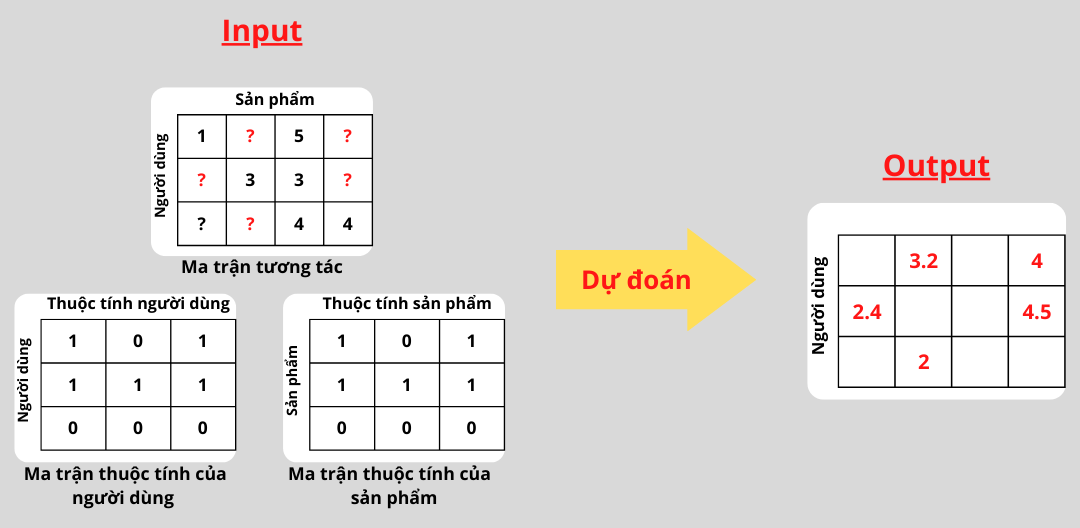
\includegraphics[width=\textwidth]{images/Chapter1/rs.png}
    \caption{Cách thức hoạt động của hệ thống đề xuất sản phẩm.}
    \label{fig:chap1_rs}
\end{figure}
Trong phạm vi đề tài của khóa luận nhóm chúng em sẽ tiến hành xử lý trên dữ liệu explicit feedback. Explicit feedback là dữ liệu cho biết rõ ràng mức độ ưa thích của người dùng đối với sản phẩm, chẳng hạn như điểm đánh giá của người dùng cho 1 bộ phim từ 1 đến 5. 


\section{Thách thức của bài toán}
\label{section:thachthuc}
Để huấn luyện được mô hình có thể đề xuất chính xác tất cả các sản phẩm cho người dùng, ta cần một bộ dữ liệu đầy đủ bao gồm đánh giá của tất cả người dùng cho tất cả sản phẩm. Tuy nhiên dữ liệu này không thể có được trong thực tế, do người dùng không thể nào xem và đánh giá tất cả các sản phẩm trong hệ thống. Vì vậy để mô hình có thể huấn luyện được tốt nhất ta cần bộ dữ liệu quan sát được phải được phát sinh từ phân phối đều của bộ dữ liệu đầy đủ này, vì bộ dữ liệu quan sát được này sẽ đại diện cho bộ dữ liệu đầy đủ và nó được gọi là dữ liệu không bị thiên lệch. 

Dữ liệu quan sát được trong bài toán đề xuất sản phẩm thường bị gặp vấn đề lớn về thiên lệch dữ liệu. Thiên lệch dữ liệu là dữ liệu quan sát được không được phát sinh từ phân phối đều, do đó nó không đại diện được cho bộ dữ liệu đầy đủ. Vấn đề thiên lệch dữ liệu bắt nguồn từ 2 nguyên nhân chính trong việc thu thập dữ liệu sau:
\begin{itemize}
    \item Do người dùng tự chọn các bộ phim để đánh giá, thay vì dựa trên việc người dùng đánh giá một tập các sản phẩm ngẫu nhiên.
    Việc người dùng đánh giá trên một tập các sản phẩm được đề xuất ngẫu nhiên sẽ đảm bảo dữ liệu thu được được phát sinh từ phân phối đều, giúp cho dữ liệu thu được có thể đại diện được cho tập dữ liệu đầy đủ.
    Một kết quả nghiên cứu của tác giả Marlin và các cộng sự \cite{bias} đã cho thấy tác động rõ ràng của thiên lệch dữ liệu. Họ đã tiến hành một cuộc khảo sát người dùng để thu thập dữ liệu điểm đánh giá của người dùng đối với một số sản phẩm được lựa chọn ngẫu nhiên, để so sánh với các sản phẩm do người dùng tự lựa chọn. Hình \ref{fig:self_selection_bias} cho thấy rõ sự khác nhau trong phân phối dữ liệu của việc lựa chọn ngẫu nhiên và do người dùng tự đánh giá; đồng thời có thể đưa ra phát hiện người dùng có xu hướng chọn và đánh giá các mặt hàng họ thích.
    \item Do hệ thống đề xuất chỉ chọn các bộ phim nào đó để hiển thị cho người dùng, trong trường hợp hệ thống đề xuất sản phẩm đã triển khai từ trước. Với tác động của hệ thống đề xuất như vậy, người dùng chỉ có thể xem và đánh giá trên các bộ phim được hiển thị, điều này làm cho dữ liệu thu thập được chỉ tập trung vào một vài loại sản phẩm nào đó, không đại diện cho toàn bộ dữ liệu.
\end{itemize}

\begin{figure}
    \centering
    \begin{subfigure}[b]{0.4\textwidth}
     \centering
     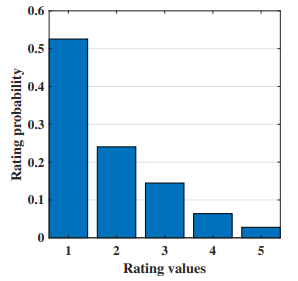
\includegraphics[width=\textwidth]{images/Chapter1/bias_1.png}
     \caption{Các sản phẩm được chọn ngẫu nhiên.}
     \label{fig:randomly_selected}
    \end{subfigure}
    \hfill
    \begin{subfigure}[b]{0.4\textwidth}
     \centering
     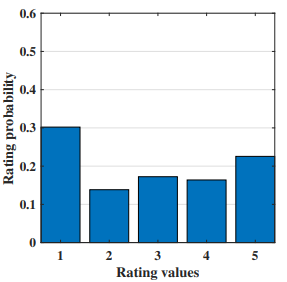
\includegraphics[width=\textwidth]{images/Chapter1/bias_2.png}
     \caption{Các sản phẩm được chọn do người dùng tự lựa chọn.}
     \label{fig:user_selected}
    \end{subfigure}
    \caption{Phân phối điểm đánh giá sản phẩm, được thu thập bằng cách cho người dùng đánh giá các sản phẩm ngẫu nhiên và cho người dùng đánh giá các sản phẩm tự lựa chọn.}
    \label{fig:self_selection_bias}
\end{figure}

Để hiểu rõ hơn về vấn đề thiên lệch dữ liệu ta sẽ xem xét một ví dụ nhỏ trong hệ thống đề xuất phim, minh họa tác động của thiên lệch dữ liệu có thể gây ra cho việc đánh giá mô hình. Hình \ref{fig:chap1_ex_1} minh họa cho thí nghiệm của ta trong đó:
\begin{itemize}
    \item Ma trận $Y$ là ma trận đầy đủ chứa đánh giá của tất cả người dùng đối với tất cả các sản phẩm, trong ma trận này bao gồm 2 nhóm nhỏ: 1) những người dùng yêu thích phim kinh dị, họ sẽ đánh giá 5 điểm cho tất cả các phim kinh dị và 1 điểm cho tất cả các phim lãng mãn mà họ đã xem; nhóm trái ngược 2) những người dùng yêu thích phim lãng mạn, họ sẽ đánh giá 1 điểm cho tất cả các phim kinh dị và 5 điểm cho tất cả các phim lãng mạn mà họ đã xem; và cả 2 nhóm người dùng đều đánh giá cho  thể loại phim kịch là 3. 
    \item Ma trận $O$ là ma trận nhị phân chứa 2 giá trị 0 và 1, đại diện cho những sản phẩm người dùng đã đánh giá trong hệ thống, \( [O_{u,i}~=~1]\Leftrightarrow[Y_{u,i} \) được quan sát].
\end{itemize}

\begin{figure}[h]
    \centering
    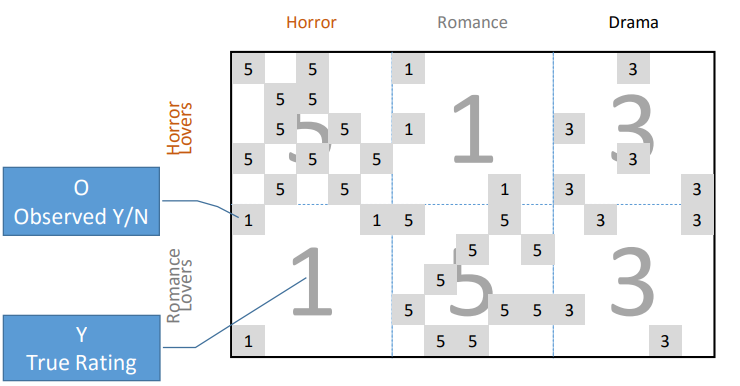
\includegraphics[width=\textwidth]{images/Chapter1/example_bias_1.png}
    \caption{Ví dụ minh họa tác động của thiên lệch dữ liệu. 
    $Y$ là những điểm đánh giá thật của dữ liệu, minh họa bằng những con số nằm bên dưới ma trận. $O$ là những sản phẩm đã được người dùng đánh giá, các sản phẩm đã được đánh giá sẽ được minh họa bằng những điểm đánh giá được bao quanh bởi ô vuông tô màu; ngược lại, các sản phẩm chưa được đánh giá thì chỉ có điểm đánh giá dự đoán.}
    \label{fig:chap1_ex_1}
\end{figure}

Xét 2 cách dự đoán $\hat{Y}_1$ và  $\hat{Y}_2$ sẽ được dùng để dự đoán giá trị cho các điểm đánh giá chưa quan sát được. Hình \ref{fig:chap1_ex_2} sẽ minh họa cách 2 mô hình dự đoán như sau:
\begin{itemize}
    \item Ở cách dự đoán $\hat{Y}_1$, những điểm đánh giá có giá trị thật là 1 sẽ được dự đoán là 5, các điểm đánh giá có giá trị thật là 3 và 5 sẽ được dự đoán đúng giá trị.
    \item Ở cách dự đoán $\hat{Y}_2$, những điểm đánh giá có giá trị thật là 3 sẽ được dự đoán là 5, các điểm đánh giá có giá trị thật là 3 và 5 sẽ được dự đoán đúng giá trị.
\end{itemize}

\begin{figure}[ht]
    \centering
    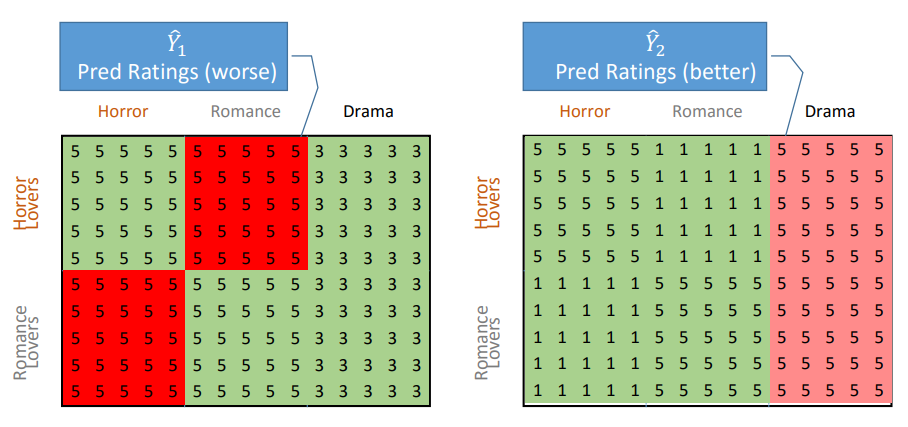
\includegraphics[width=\textwidth]{images/Chapter1/example_bias_2.png}
    \caption{Các cách dự đoán $\hat{Y}_1$ và $\hat{Y}_2$ trên tập dữ liệu. Nhìn vào hình thì cách dự đoán $\hat{Y}_2$ tốt hơn cách dự đoán $\hat{Y}_1$.}
    \label{fig:chap1_ex_2}
\end{figure}

Nếu chúng ta có thể quan sát toàn bộ dữ liệu như trong hình \ref{fig:chap1_ex_2}, ta có thể thấy với cách dự đoán $\hat{Y}_1$ khi giá trị thật là 1 nhưng dự đoán là 5 thì độ lỗi của nó rất lớn. Khi so với cách dự đoán $\hat{Y}_2$ khi giá trị thật là 3 và dự đoán là 5 có độ lỗi không quá nghiêm trọng như cách dự đoán $\hat{Y}_1$.

Để đánh giá một cách dự đoán có tốt hay không, ta sẽ tiến hành đánh giá độ lỗi trên tập dữ liệu quan sát được. Tuy nhiên dữ liệu quan sát được ở đây lại không được phát sinh từ phân phối đều do đó nó có sự thiên lệch, cụ thể hơn là những điểm đánh giá là 1 xuất hiện ít hơn những điểm đánh giá là 3 (minh họa ở hình \ref{fig:chap1_ex_3}); điều này bắt nguồn từ việc người dùng tự lựa chọn các bộ phim họ thích để đánh giá.

Khi đánh giá cách dự đoán nào là tốt trên tập dữ liệu quan sát được bị thiên lệch này, ta sẽ cho rằng dự đoán $\hat{Y}_1$ tốt hơn $\hat{Y}_2$. Vì theo cách dự đoán $\hat{Y}_1$ những điểm có độ lỗi lớn (điểm đánh giá thật là 1 nhưng dự đoán là 5) xuất hiện rất ít trong bộ dữ liệu quan sát được; trong khi đó theo cách dự đoán $\hat{Y}_2$ những điểm có độ lỗi nhỏ hơn (điểm đánh giá thật là 3 nhưng dự đoán là 5) xuất hiện nhiều hơn trong bộ dữ liệu quan sát được; điều này làm cho độ lỗi của cách dự đoán $\hat{Y}_1$ thấp hơn cách dự đoán $\hat{Y}_2$ mặc dù cách dự đoán $\hat{Y}_1$ tệ hơn. 

\begin{figure}[h]
    \centering
    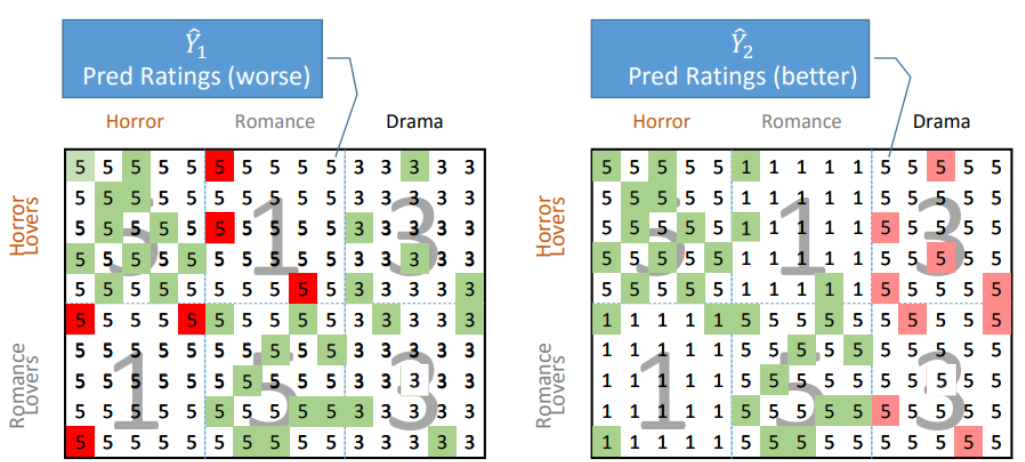
\includegraphics[width=\textwidth]{images/Chapter1/example_bias_3.png}
    \caption{Đánh giá 2 mô hình dự đoán $\hat{Y}_1$, $\hat{Y}_2$ dựa trên các mẫu quan sát được.}
    \label{fig:chap1_ex_3}
\end{figure}

\section{Phương pháp giải quyết bài toán mà nhóm em tìm hiểu}
Để khắc phục vấn đề thiên lệch dữ liệu tác giả Tobias Schnabel và các cộng sự \cite{IPS} trong bài báo ``Recommendations as Treatments: Debiasing Learning and Evaluation'' tại hội nghị ``ICML 2016'', đã đề xuất việc áp dụng phương pháp ``Inverse Propensity Scoring'' (IPS) vào quá trình huấn luyện và đánh giá mô hình. IPS hoạt động bằng cách đánh lại trọng số của các mẫu dựa trên propensity, theo cách giảm trọng số của các mẫu thường quan sát được, trong khi tăng trọng số của các mẫu hiếm gặp. Điều này sẽ giúp kiểm soát được vấn đề thiên lệch của dữ liệu.

\section{Bố cục}
Phần còn lại của khóa luận sẽ được trình bày như sau:
\begin{itemize}
    \item Chương 2 trình bày kiến thức nền tảng về ``Matrix Factorization'', ``Gradient Descent'', ``Naive Bayes'' và ``Logistic Regression''.
    \item Chương 3 trình bày về độ đo IPS và ứng dụng của nó trong việc đánh giá và huấn luyện mô hình; đây là phần chính của khóa luận. Trong phần này gồm có hai phần nhỏ:
    \begin{itemize}
        \item Ước lượng propensity: nhóm chúng em trình bày về cách ước lượng ma trận propensity thông qua 2 mô hình ``Naive Bayes'' và ``Logistic Regression''.
        \item Sử dụng phương pháp ``Matrix Factorization'' kết hợp với propensity vừa tìm được và các vấn đề cần lưu ý của phương pháp này.
    \end{itemize}
    \item Chương 4 trình bày về các thí nghiệm và các kết quả đạt được.
    \item Cuối cùng, tổng kết và các hướng phát triển sẽ được trình bày ở chương 5.
\end{itemize}
